\documentclass{tietreport}

% Prevent blank pages after the title page
\let\cleardoublepage\clearpage

\usepackage{graphicx}
\usepackage{float}
\usepackage{longtable}
\usepackage{array}
\usepackage{booktabs}
\usepackage{enumitem}

\newcolumntype{L}[1]{>{\raggedright\arraybackslash}p{#1}}
\setlength{\headheight}{15pt}
% Allow long identifiers such as table names to break after underscores
\renewcommand{\_}{\textunderscore\allowbreak}
\setlength{\emergencystretch}{3em}

% Numbered sections (1., 1.1, 1.1.1) instead of chapters,
% matching the project proposal
\renewcommand{\thesection}{\arabic{section}}
\titleformat{\section}
  {\Large\bfseries}
  {\thesection.}
  {0.5em}
  {}
\titleformat{\subsection}
  {\large\bfseries}
  {\thesubsection}
  {0.5em}
  {}

% ==================================================
% TITLE PAGE
% ==================================================

\TitlePageHeader{%
  UCS503 - Software Engineering
}

\ProjectTitle{%
  GATED: Apartment Tracker
}

\ProjectSubTitle{%
  A Smart Digital Platform for Apartment and Society Management
}

\author{%
  \texttt{1024030101} Khushi Dangi \\
  \texttt{1024030115} Geetika Parakh \\
  \texttt{1024030121} Ridham Sharma \\
  \texttt{1024030937} Harnoor Singh
}

\TitlePageSubText{%
  Group: \texttt{3C14} \\
  BE Third Year, CSE
}

\AdvisorName{%
  Anushka
}

\TitlePageFooterText{{%
    \large Final Project Report \\[0.2cm]
    \bfseries Computer Science and Engineering Department
  } \\[0.15cm]
  Thapar Institute of Engineering and Technology, Patiala%
}

% ==================================================

\begin{document}

\maketitle

\tableofcontents

\newpage

% ==================================================
% 1. INTRODUCTION
% ==================================================

\section{Introduction}

\subsection{Background}

Residential societies bring together residents, society administrators,
security guards, and maintenance staff. Many societies still manage
day-to-day work through paper registers, phone calls, spreadsheets, and
messaging groups. Complaints are hard to track, visitor records are kept in
physical books, maintenance bills are prepared by hand, and facility bookings
often clash.

GATED: Apartment Tracker is a mobile and web application that brings these
activities onto one platform. Every user signs in with their own account and
sees only the features and data that match their role and society.

\subsection{Problem Statement}

The project proposal identified the following problems with manual society
management:

\begin{itemize}
  \item \textbf{Fragmented communication:} requests and notices are spread
  across many channels.
  \item \textbf{Delayed complaint resolution:} complaints are difficult to
  assign and follow up.
  \item \textbf{Poor transparency:} residents cannot see the status of their
  complaints or payments.
  \item \textbf{Manual visitor management:} physical registers slow down
  verification at the gate.
  \item \textbf{Billing errors:} hand-made maintenance bills lead to
  inconsistencies.
  \item \textbf{Booking conflicts:} manual facility reservations can overlap.
\end{itemize}

GATED addresses these problems with a centralised, role-based application
backed by a single database.

\subsection{Objectives}

\begin{enumerate}
  \item Provide a centralised platform for residents, administrators,
  security guards, and maintenance staff.
  \item Allow residents to register against a verified society and apartment,
  and sign in securely.
  \item Simplify complaint registration, assignment, and tracking.
  \item Publish society notices digitally.
  \item Provide conflict-free facility booking.
  \item Provide transparent maintenance billing and payment status.
  \item Support visitor requests and gate management.
  \item Protect user and society data through role-based access control.
\end{enumerate}

\subsection{Scope of the Final Deliverable}

The final version delivers authentication with society and apartment
verification, role-based dashboards for all four roles, the complete
complaint lifecycle, the notice board, facility booking, and maintenance
billing, all backed by Supabase with Row Level Security. Visitor management is
available as a user interface prototype. Parking management, notifications,
and QR visitor passes are left for future work
(Section~\ref{sec:future}).

% ==================================================
% 2. REQUIREMENTS
% ==================================================

\section{Requirements Specification}

\subsection{Stakeholders and User Roles}

\begin{longtable}{L{3.2cm} L{10.6cm}}
\toprule
\textbf{Role} & \textbf{Responsibilities in the system} \\
\midrule
\endhead
Resident & Registers against a society and apartment, raises complaints and
maintenance requests, tracks their status, reads notices, books facilities,
views and pays maintenance bills, requests visitor passes. \\
Society Admin & Views all complaints of the society, assigns them to
maintenance staff, publishes and deletes notices, creates maintenance bills,
views all facility bookings. \\
Maintenance Staff & Views complaints assigned to them, starts work, and
resolves complaints with a resolution note. \\
Security Guard & Uses the security dashboard to manage visitors and read
notices. \\
\bottomrule
\end{longtable}

\subsection{Functional Requirements}

\begin{longtable}{L{1.4cm} L{12.4cm}}
\toprule
\textbf{ID} & \textbf{Requirement} \\
\midrule
\endhead
FR-1 & Users shall register and sign in with email and password. Residents
shall select a registered society and enter an apartment number that exists
in that society's registry. \\
FR-2 & After sign-in, users shall be routed to the dashboard for their role. \\
FR-3 & Residents shall raise complaints and maintenance requests with a
subject, category, priority, and description, and track their status. \\
FR-4 & Administrators shall view all complaints of their society and assign
a complaint to a maintenance staff member. \\
FR-5 & Maintenance staff shall view assigned complaints and move them from
\textit{assigned} to \textit{in progress} to \textit{resolved}, adding a
resolution note. \\
FR-6 & Administrators shall publish notices with a priority (General,
Important, Urgent); all members of the same society shall be able to read
them. \\
FR-7 & Residents shall book society facilities for a future time slot; the
system shall prevent overlapping bookings of the same facility. \\
FR-8 & Administrators shall create one maintenance bill per flat per month;
residents shall view their flat's bills and record payment. \\
FR-9 & Residents shall request visitor passes, and security staff shall
verify visitor entry. \\
\bottomrule
\end{longtable}

\subsection{Non-Functional Requirements}

\begin{longtable}{L{1.6cm} L{12.2cm}}
\toprule
\textbf{ID} & \textbf{Requirement} \\
\midrule
\endhead
NFR-1 & \textbf{Security:} data access shall be restricted by role and
society using database-level Row Level Security, not only by hiding screens.
Only resident accounts may self-register. \\
NFR-2 & \textbf{Portability:} the application shall run on Android, iOS, and
the web from a single code base. \\
NFR-3 & \textbf{Correctness:} business rules such as no double booking and
one bill per flat per month shall be enforced in the database. \\
NFR-4 & \textbf{Usability:} each form shall validate input and show a clear
message when something is wrong. \\
NFR-5 & \textbf{Maintainability:} the code shall be modular, typed with
TypeScript, and the database shall be reproducible from migration files. \\
\bottomrule
\end{longtable}

% ==================================================
% 3. SYSTEM DESIGN
% ==================================================

\section{System Design}

\subsection{System Architecture}

GATED follows a client--server architecture. The Expo (React Native)
application is the client and runs on mobile devices and in the browser.
Supabase is the backend and provides authentication, a PostgreSQL database,
Row Level Security (RLS) policies, and server-side functions (RPCs).
Business rules that must not be bypassed, such as booking overlap checks and
bill creation, run inside the database, so the rules hold even if a client
sends requests directly to the API.

\begin{center}
Mobile / Web client (Expo Router screens)
$\rightarrow$
Supabase Auth + REST API
$\rightarrow$
PostgreSQL (RLS policies, triggers, RPC functions)
\end{center}

\subsubsection*{Application Flow}

\begin{center}
Sign Up $\rightarrow$ Society Selection $\rightarrow$ Apartment Verification
$\rightarrow$ Account Creation $\rightarrow$ Sign In $\rightarrow$
Role Lookup $\rightarrow$ Role-Based Dashboard
\end{center}

The complaint workflow follows:

\begin{center}
Resident submits $\rightarrow$ \textit{submitted} $\rightarrow$ Admin assigns
$\rightarrow$ \textit{assigned} $\rightarrow$ Staff starts work $\rightarrow$
\textit{in progress} $\rightarrow$ Staff resolves with note $\rightarrow$
\textit{resolved}
\end{center}

\subsection{Use Case Diagram}

\begin{figure}[H]
    \centering
    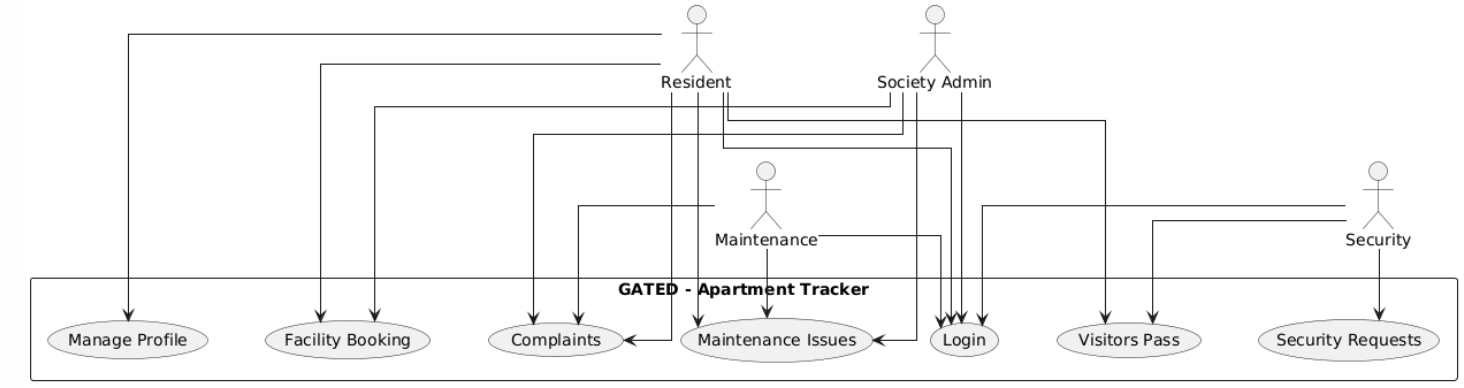
\includegraphics[width=0.9\textwidth]{use_case_diagram.png}
    \caption{Use Case Diagram of GATED: Apartment Tracker}
    \label{fig:usecase}
\end{figure}

\subsection{UML Class Diagram}

\begin{figure}[H]
    \centering
    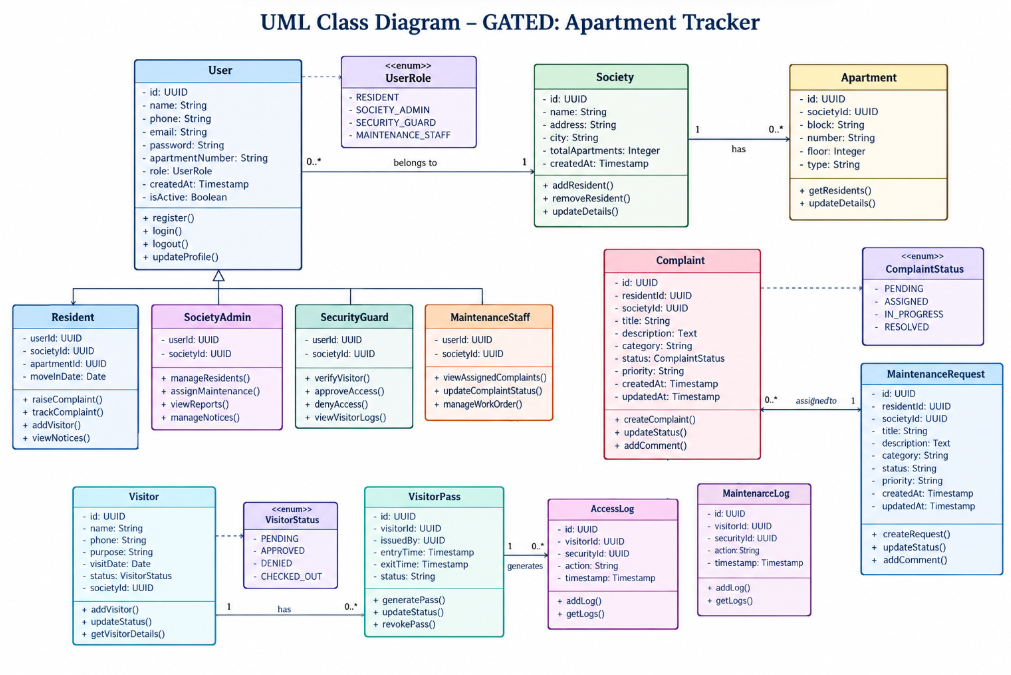
\includegraphics[width=\textwidth]{class_diagram.png}
    \caption{UML Class Diagram}
    \label{fig:class}
\end{figure}

\subsection{UML Sequence Diagram}

\begin{figure}[H]
    \centering
    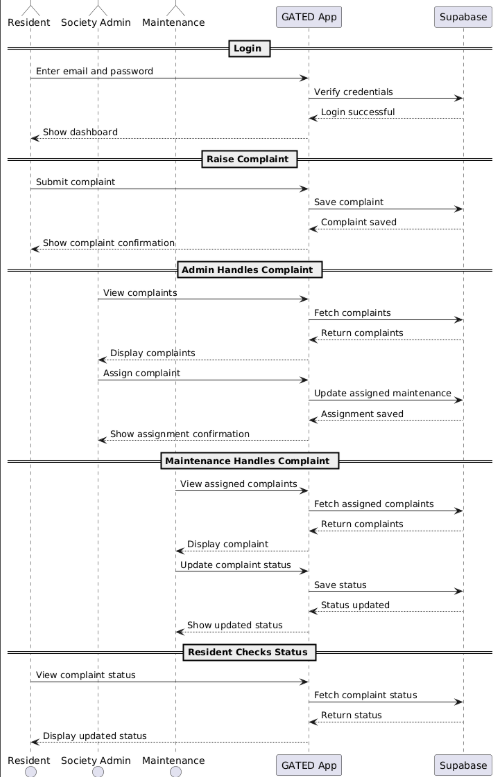
\includegraphics[width=\textwidth, height=0.7\textheight,
      keepaspectratio]{sequence_diagram.png}
    \caption{UML Sequence Diagram}
    \label{fig:sequence}
\end{figure}

\subsection{Database Design}

\begin{figure}[H]
    \centering
    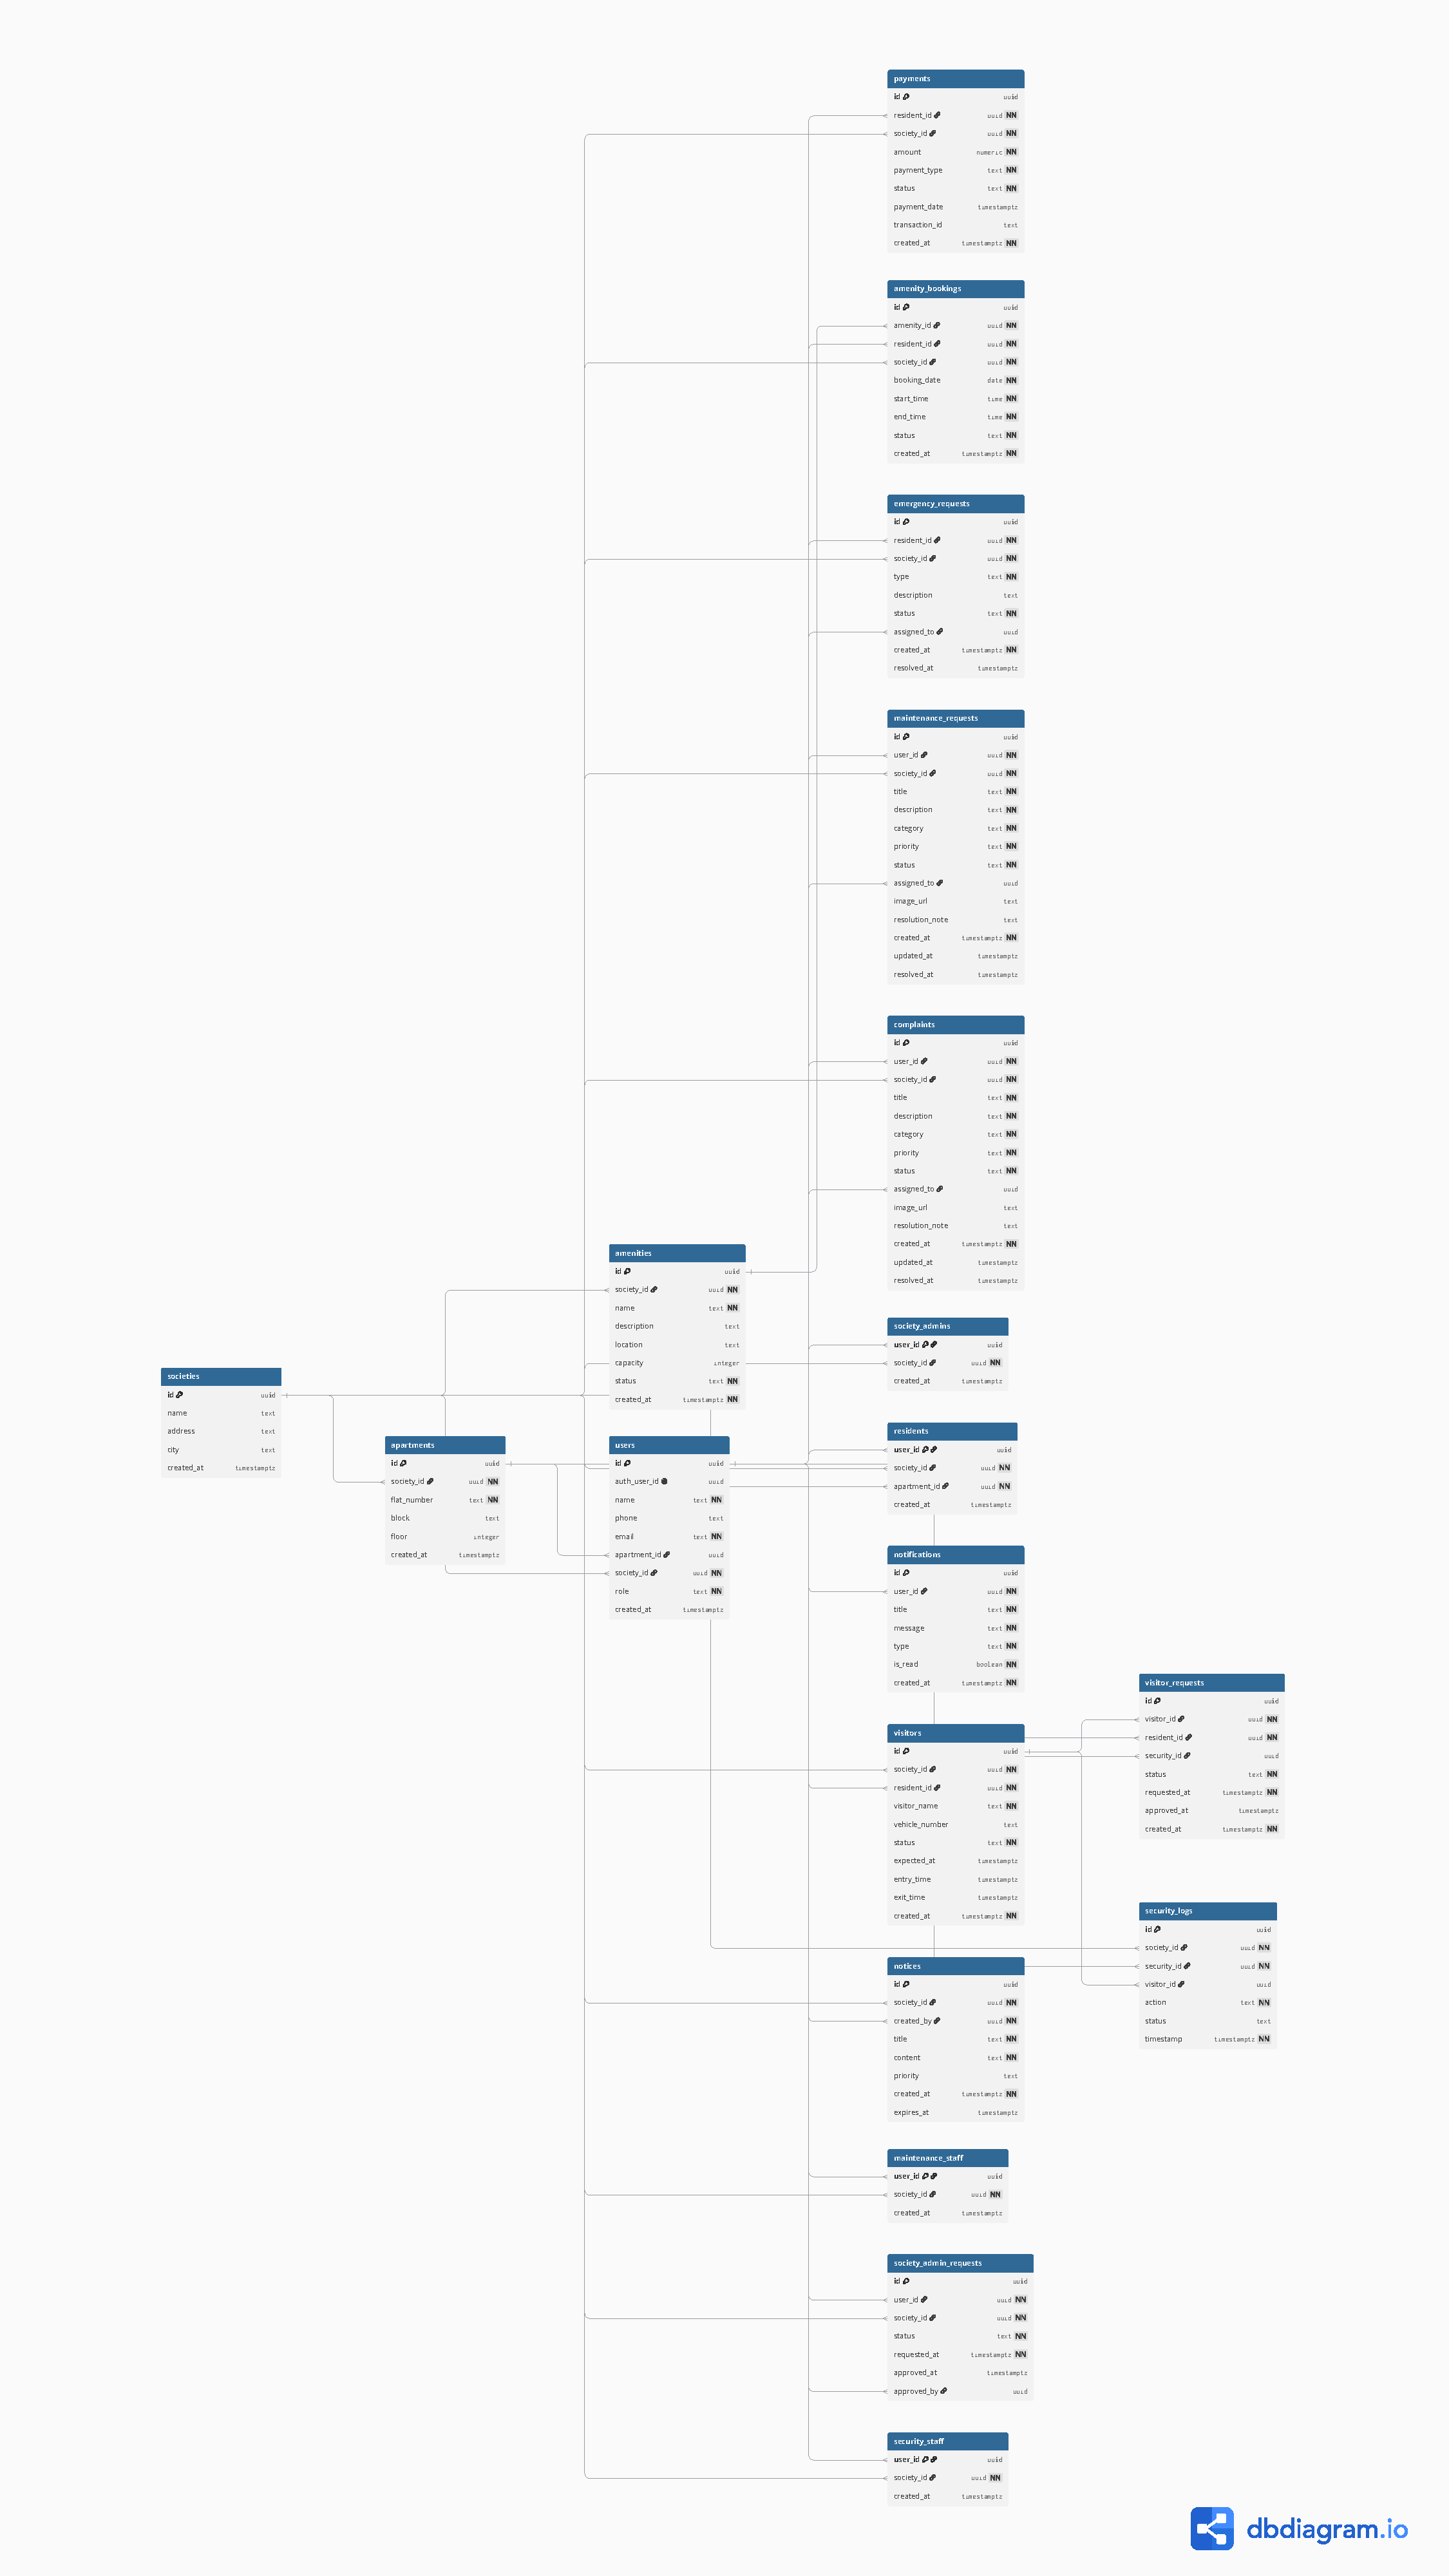
\includegraphics[width=\textwidth, height=0.7\textheight,
      keepaspectratio]{er_diagram.pdf}
    \caption{Entity Relationship Diagram}
    \label{fig:er}
\end{figure}

The core entities are \texttt{societies}, \texttt{apartments},
\texttt{users}, \texttt{complaints}, and \texttt{maintenance\_requests}.
In the final phase three tables were added through the migration
\texttt{20261124120000\_apartment\_services.sql}:

\begin{longtable}{L{4cm} L{9.8cm}}
\toprule
\textbf{Table} & \textbf{Purpose and key constraints} \\
\midrule
\endhead
\texttt{apartment\_notices} & Society-scoped notices. Title 1--100
characters, body 1--2000 characters, priority is General, Important, or
Urgent. \\
\texttt{facility\_reservations} & Bookings for Gym, Clubhouse, Swimming
Pool, Community Hall, and Tennis Court. \texttt{end\_at > start\_at}; status
is BOOKED or CANCELLED. \\
\texttt{maintenance\_bills} & Bills per apartment. Amount must be positive,
billing month is the first day of a month, status is PENDING or PAID, and
\texttt{UNIQUE(apartment\_id, billing\_month)} allows one bill per flat per
month. \\
\bottomrule
\end{longtable}

\subsection{Security Design}

\begin{itemize}
  \item \textbf{Authentication:} Supabase Auth with email and password.
  Sessions are stored in AsyncStorage on mobile and in local storage on the
  web.
  \item \textbf{Controlled registration:} the
  \texttt{lookup\_signup\_apartment} function checks one apartment number
  without exposing the apartment table. The \texttt{handle\_gated\_signup}
  trigger creates the profile on the server, and
  \texttt{enforce\_resident\_self\_signup} rejects any self-signup that is
  not a resident. Staff accounts are provisioned through the Supabase Admin
  API.
  \item \textbf{Row Level Security:} every new table has RLS enabled.
  Notices are readable by members of the same society and writable only by
  its admin. Residents read only their own bookings and their own flat's
  bills; admins read all records of their society.
  \item \textbf{Server-side business rules:} the
  \texttt{guard\_facility\_reservation} trigger rejects past start times and
  overlapping bookings and takes an advisory lock per facility so that two
  simultaneous requests cannot both succeed. Bills are created and paid only
  through \texttt{SECURITY DEFINER} functions that check the caller's role.
\end{itemize}

% ==================================================
% 4. IMPLEMENTATION
% ==================================================

\section{Implementation}

\subsection{Technology Stack}

\begin{longtable}{L{4cm} L{9.8cm}}
\toprule
\textbf{Layer} & \textbf{Technology} \\
\midrule
\endhead
Framework & React Native 0.86 with Expo SDK 57 \\
Language & TypeScript \\
Navigation & Expo Router (file-based routing, typed routes) \\
Backend & Supabase (PostgreSQL, Auth, REST, RPC) \\
Security & Supabase Row Level Security, database triggers \\
Storage & AsyncStorage (mobile), browser local storage (web) \\
Tools & Visual Studio Code, Expo Go, Git and GitHub, LaTeX \\
\bottomrule
\end{longtable}

\subsection{Project Structure}

\begin{longtable}{L{4.6cm} L{9.2cm}}
\toprule
\textbf{Path} & \textbf{Contents} \\
\midrule
\endhead
\texttt{src/app/} & Screens, one file per route (sign-in, signup steps,
dashboards, complaints, notices, bills, facility booking, visitors,
profile). \\
\texttt{src/components/} & Shared components: navigation menu, admin
complaint card and assignment modal, resident dashboard cards. \\
\texttt{src/lib/} & Supabase client and the in-memory signup draft. \\
\texttt{src/constants/}, \texttt{src/styles/} & Complaint categories and
statuses, theme colours, and shared styles. \\
\texttt{supabase/} & SQL migrations and seed data. \\
\texttt{docs/} & Database schema, project selection criteria, test cases. \\
\bottomrule
\end{longtable}

\subsection{Module Implementation}

\begin{itemize}
  \item \textbf{Authentication and roles:} signup validates the email,
  phone (7--15 digits), and password (at least 6 characters), then checks
  the chosen society and apartment number against the registry before
  creating the account. On sign-in the user's role decides which dashboard
  opens, and each dashboard checks the role again.
  \item \textbf{Complaints:} residents submit complaints or maintenance
  requests with one of eleven categories and a priority. Admins assign them
  to maintenance staff, who start work and resolve them with a required
  resolution note. Residents follow the status on their dashboard.
  \item \textbf{Notice board:} admins publish notices with a priority and
  can delete them; all members of the society can read them.
  \item \textbf{Facility booking:} residents book one of five facilities
  for a future slot; overlaps are rejected in the app and again in the
  database. Bookings can be cancelled.
  \item \textbf{Maintenance billing:} admins create one bill per flat per
  month; residents see their flat's bills and record a simulated payment.
  \item \textbf{Visitor management:} residents fill in a visitor pass
  request, which is currently shown on screen but not yet saved.
\end{itemize}

% ==================================================
% 5. TESTING
% ==================================================

\section{Testing}

\subsection{Testing Strategy}

The application was tested at four levels:

\begin{itemize}
  \item \textbf{Static analysis:} the TypeScript compiler checks the whole
  code base (\texttt{npx tsc --noEmit}).
  \item \textbf{Functional and validation testing:} each screen is tested
  with valid input, invalid input, and boundary values (for example a
  6-character password, a 7- and 15-digit phone number, a back-to-back
  booking, an amount of zero).
  \item \textbf{Integration testing:} complete workflows that cross roles,
  such as a complaint moving from a resident to an admin to maintenance staff
  and back to the resident.
  \item \textbf{Security testing:} attempts to read or change data that
  belongs to another role, user, or society, both through the app and by
  calling the Supabase API directly with a user's session.
\end{itemize}

\subsection{Test Environment}

\begin{itemize}
  \item Client: Expo Go on Android, and the web build in a desktop browser.
  \item Backend: Supabase project with both migrations and
  \texttt{supabase/seed.sql} applied (five societies, flats A-101, A-102,
  B-201, B-202).
  \item Accounts: two residents of Lakeview Gardens (flats A-101 and A-102),
  one resident of another society, and one admin, maintenance staff member,
  and security guard of Lakeview Gardens.
\end{itemize}

\subsection{Test Case Summary}

The full set of 92 test cases, with pre-conditions, steps, test data, and
expected results, is maintained in \texttt{docs/test-cases.md}.

\begin{longtable}{L{5.2cm} L{3cm} L{5.4cm}}
\toprule
\textbf{Module} & \textbf{Test IDs} & \textbf{Requirements covered} \\
\midrule
\endhead
Registration & TC-01 -- TC-21 & FR-1, NFR-1, NFR-4 \\
Sign in, routing, sign out & TC-22 -- TC-31 & FR-1, FR-2, NFR-1 \\
Complaints and maintenance & TC-32 -- TC-48 & FR-3, FR-4, FR-5, NFR-1 \\
Notice board & TC-49 -- TC-55 & FR-6, NFR-1 \\
Facility booking & TC-56 -- TC-68 & FR-7, NFR-3 \\
Maintenance billing & TC-69 -- TC-81 & FR-8, NFR-3 \\
Visitor management & TC-82 -- TC-85 & FR-9 \\
Profile and navigation & TC-86 -- TC-87 & FR-2 \\
Non-functional & TC-88 -- TC-92 & NFR-2, NFR-5 \\
\midrule
\textbf{Total} & \textbf{92} & \\
\bottomrule
\end{longtable}

% ==================================================
% 6. RESULTS AND DISCUSSION
% ==================================================

\section{Results and Discussion}

\subsection{Requirements Traceability}

\begin{longtable}{L{4.2cm} L{2.6cm} L{6.8cm}}
\toprule
\textbf{Proposed module} & \textbf{Status} & \textbf{Notes} \\
\midrule
\endhead
Authentication and role management & Implemented & Society and apartment
verification, server-side profile creation, resident-only self-signup,
role-based routing. \\
Apartment and resident management & Partial & Apartment registry is used
for verification; admins cannot yet add or edit residents from the app. \\
Complaint management & Implemented & Full lifecycle with assignment and
resolution notes. \\
Notice board & Implemented & Priorities, society scoping, admin delete. \\
Facility booking & Implemented & Overlap prevention in the app and in the
database, cancellation. \\
Maintenance billing & Implemented (simulated payment) & One bill per flat
per month, totals, payment status. \\
Visitor management & Partial & Request form prototype; not saved; no QR
pass yet. \\
Analytics dashboard & Partial & Complaint counts and bill totals on
dashboards. \\
Parking management & Not implemented & Future work. \\
Notifications & Not implemented & Future work. \\
\bottomrule
\end{longtable}

\subsection{Evaluation Against Proposed Metrics}

\begin{itemize}
  \item \textbf{Complaint processing time:} every complaint records
  \texttt{created\_at}, \texttt{updated\_at}, and \texttt{resolved\_at}, so
  the time from submission to assignment and resolution can be measured
  directly from the database.
  \item \textbf{Booking conflict rate:} overlapping bookings of the same
  facility are rejected by the database trigger under a per-facility lock,
  so the expected conflict rate is zero (verified by TC-60, TC-61, and
  TC-64).
  \item \textbf{Visitor verification time:} cannot be measured yet because
  visitor requests are not stored.
  \item \textbf{Workflow completion:} five core workflows (signup,
  complaints, notices, facility bookings, and bills) can be completed end to
  end; the visitor workflow cannot yet.
\end{itemize}

\subsection{Challenges Faced}

\begin{itemize}
  \item \textbf{Profile creation with email confirmation:} an unconfirmed
  user has no session and cannot insert their own profile. This was solved
  with a database trigger on \texttt{auth.users}.
  \item \textbf{Preventing privilege escalation:} signup metadata is set by
  the client, so a user could claim to be an admin. A second trigger now
  accepts only resident self-signups.
  \item \textbf{Double booking under RLS:} a resident cannot see other
  residents' bookings, so a client-side check alone is not enough. The
  overlap check was moved into a database trigger.
  \item \textbf{Approval flow:} an earlier admin-approval step blocked new
  residents from using the app; it was removed in favour of apartment
  registry verification.
\end{itemize}

% ==================================================
% 7. LIMITATIONS AND FUTURE SCOPE
% ==================================================

\section{Limitations and Future Scope}
\label{sec:future}

\subsection{Current Limitations}

\begin{itemize}
  \item Visitor requests are kept only in the screen's state, so they are
  lost when the app reloads and are not visible to security staff.
  \item The security dashboard has tiles for Deliveries, Gate activity,
  Residents, and Emergency whose screens are not built yet.
  \item The ``society not listed'' contact form does not save or send the
  request.
  \item Bill payment is simulated; no payment gateway is connected.
  \item Facility booking times are typed as text in
  \texttt{YYYY-MM-DDTHH:mm} format instead of using a date picker.
  \item The table definitions and RLS policies for \texttt{complaints} and
  \texttt{maintenance\_requests} were created in the Supabase dashboard and
  are not yet captured in the repository's migration files.
  \item There is no automated unit or end-to-end test suite; testing is
  manual.
\end{itemize}

\subsection{Future Scope}

\begin{enumerate}
  \item Store visitor requests in the \texttt{visitors} and
  \texttt{visitor\_requests} tables and issue QR passes with an expiry time.
  \item Build the remaining security screens: deliveries, gate activity
  log, resident directory, and emergency alerts.
  \item Push notifications for complaint updates, visitors, and new
  notices.
  \item Online payment of maintenance bills through a payment gateway.
  \item Parking allocation for residents and visitors.
  \item An analytics dashboard for administrators showing complaint
  resolution times, collections, and facility usage.
  \item Admin screens to manage apartments, residents, and staff.
  \item Automated tests with Jest and React Native Testing Library, and
  database policy tests.
\end{enumerate}

% ==================================================
% 8. CONCLUSION
% ==================================================

\section{Conclusion}

GATED: Apartment Tracker shows that the routine work of a residential society
can be brought onto a single role-based platform. Residents register against
a verified apartment, raise and follow complaints, read notices, book
facilities without clashes, and see their maintenance bills. Administrators
assign complaints, publish notices, and generate bills, and maintenance staff
update the complaints assigned to them.

Building the system on Expo and Supabase gave one code base for mobile and
web and allowed the important rules to be enforced inside the database
through Row Level Security, triggers, and server-side functions. The project
gave the team practical experience with requirements engineering, system
design, database design, security, testing, version control, and
documentation. Completing the visitor module, notifications, and online
payments would turn the prototype into a complete society management
solution.

% ==================================================
% REFERENCES
% ==================================================

\section*{References}
\addcontentsline{toc}{section}{References}

\begin{enumerate}[label={[\arabic*]}]
  \item Expo, \textit{Expo SDK 57 Documentation},
  \url{https://docs.expo.dev/versions/v57.0.0/}.
  \item Meta Platforms, \textit{React Native Documentation},
  \url{https://reactnative.dev/docs/getting-started}.
  \item Supabase, \textit{Supabase Documentation: Auth, Database and Row
  Level Security}, \url{https://supabase.com/docs}.
  \item The PostgreSQL Global Development Group, \textit{PostgreSQL
  Documentation: Row Security Policies and Triggers},
  \url{https://www.postgresql.org/docs/}.
  \item R. S. Pressman and B. R. Maxim, \textit{Software Engineering: A
  Practitioner's Approach}, 9th ed., McGraw-Hill, 2019.
  \item I. Sommerville, \textit{Software Engineering}, 10th ed., Pearson,
  2015.
\end{enumerate}

\end{document}
